\documentclass[addpoints]{exam}

\usepackage{amsmath}
\usepackage{amssymb}
\usepackage{graphbox}
\usepackage{graphicx}
\usepackage{hyperref}
\usepackage{tabularx}
\usepackage{tikz}
\usepackage{titling}
\usepackage{makecell}

\graphicspath{{images//}}

\tikzstyle{arrow} = [->,>=stealth]
\tikzstyle{node} = [auto,font=\footnotesize,draw,circle]

% Header and footer.
\pagestyle{headandfoot}
\runningheadrule
\runningfootrule
\runningheader{CS 412 Algorithms, Spring 2022}{Homework 2}{\theauthor}
\runningfooter{}{Page \thepage\ of \numpages}{}
\firstpageheader{}{}{}

\boxedpoints
\printanswers

\title{Homework 2\\ CS 412 Algorithms: Design and Analysis}
\author{$<$\textit{team-name}$>$}  % replace with your team name without the brackets, e.g. upper-bound
\date{Habib University, Spring 2022}

\begin{document}
\maketitle

\begin{questions}

  \section*{Network Flow}

\question \begin{tabularx}{\textwidth}{cX}
    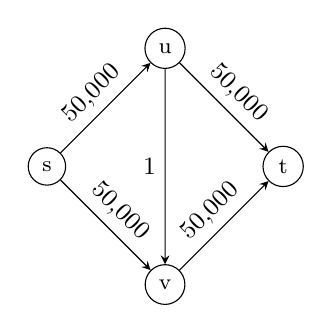
\begin{tikzpicture}[scale=1.5,baseline=(current bounding box.center)]
      \small
      \node[node] at (0,0) (s) {s};
      \node[node] at (2,0) (t) {t};
      \node[node] at (1,1) (u) {u};
      \node[node] at (1,-1) (v) {v};

      \draw[arrow] (s) -- (v) node[midway,above, sloped]{50,000};
      \draw[arrow] (s) -- (u) node[midway,above, sloped]{50,000};
      \draw[arrow] (v) -- (t) node[midway,above, sloped]{50,000};
      \draw[arrow] (u) -- (t) node[midway,above, sloped]{50,000};
      \draw[arrow] (u) -- (v) node[midway,left]{1};
    \end{tikzpicture}
    &
    \parbox[c]{\linewidth}{Argue why the Ford-Fulkerson method will not terminate in $O(VE^2)$ time for the flow network on the left. How much time will it take instead? And how can this be improved?}
  \end{tabularx}

  \begin{solution}
    
  \end{solution}
  \section*{Dynamic Programming}
\question
  \begin{tabularx}{\textwidth}{cX}
    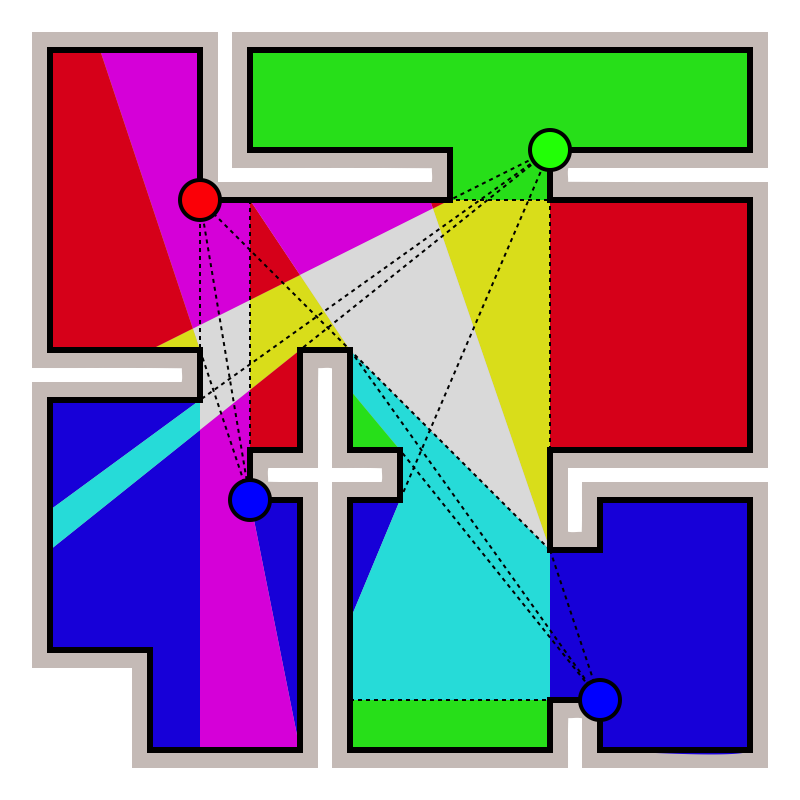
\includegraphics[width=.2\textwidth,align=t]{gallery}
    &
    Consider a version of the \href{https://en.wikipedia.org/wiki/Art_gallery_problem}{art gallery problem} where the layout of the gallery is a graph, one or more artworks are placed at each node, and edges represent corridors. Placing a security camera at a node \textit{covers} the artworks at the node and its neighbors. Design a linear-time dynamic programming approach to find the minimum number of security cameras needed to cover all the artworks. Furthermore, determine the nodes at which cameras need to be placed in the gallery whose \href{https://rpruim.github.io/m252/S19/from-class/graphs/graph-representations.html}{edge list representation} is: $\{[n_1,n_2], [n_1, n_3], [n_2,n_4], [n_2, n_5],[n_3,n_6], [n_5, n_7],[n_5,n_8]\}$.\\
    \href{https://en.wikipedia.org/wiki/Art_gallery_problem}{Wikipedia}
  \end{tabularx}
  
  \begin{solution}
    
  \end{solution}

\question
  \begin{tabularx}{\textwidth}{cX}
    
\includegraphics[scale=.15,align=t]{elements}
    &
    HU has had a successful round of fundraising and has five million to allocate to new courtyards. Up to three courtyards are planned and tenders have been invited from different architects for each courtyard. Each proposal has to include the proposed cost of construction and the potential \href{https://www.sparknotes.com/lit/bravenew/key-questions-and-answers/}{\textit{soma}}\footnote{See, ``What is soma?''} score.

    The following table shows the received proposals. Using dynamic programming, find the optimal allocation of five million that maximizes the total soma score. Any amount not allocated out of 5 million is lost.
    \\
    \href{https://ar.pinterest.com/pin/296745062922984411/}{Pinterest}
  \end{tabularx}

  \begin{center}
    \begin{tabular}{|l|*{6}{c|}}
      \hline
      & \multicolumn{2}{|c|}{Light courtyard} & \multicolumn{2}{|c|}{Flow courtyard} & \multicolumn{2}{|c|}{Nirvana courtyard} \\\hline
      &Cost& Soma & Cost & Soma & Cost& Soma \\\hline\hline
      Alpha Developers & 1M & 5 & 2M & 8 & 1M & 4 \\\hline
      Yohsin Dreams &  &  & 2M & 6 & 3M & 9 \\\hline
      High, Bar \& Exit  &  &  & 4M & 12 &  &  \\\hline
    \end{tabular}
  \end{center}  
  \noindent\underline{Hint}: Break the problem into three stages, where each stage represents the money allocated to a single courtyard. For instance, stage 1 represents the money allocated to Light courtyard, and so on. You may assume a specific ordering for the three stages, e.g. allocating to Light courtyard first, then Flow, and then Nirvana. 

  \begin{solution}
    
  \end{solution}

\question
  \begin{tabularx}{\textwidth}{lXr}
    \makecell[t]{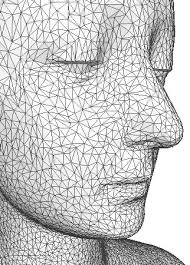
\includegraphics[width=.2\textwidth,align=t]{mesh}\\\href{http://glasnost.itcarlow.ie/~powerk/GeneralGraphicsNotes/meshes/polygon_meshes_old.html}{\small 3D Object Representations}}
    &
    Modern rendering hardware is optimized for triangles. Any 3D object to be rendered has to be \textit{triangulated}, because of which the \textit{triangle mesh} is the de-facto choice of representation for 3D objects. It is known that any polygon can be triangulated, however the number of triangulations is not generally unique. Devise a dynamic programming approach to compute the number of triangulations of a polygon with $n$ vertices. Argue about the complexity of your approach.
    &
    \makecell[t]{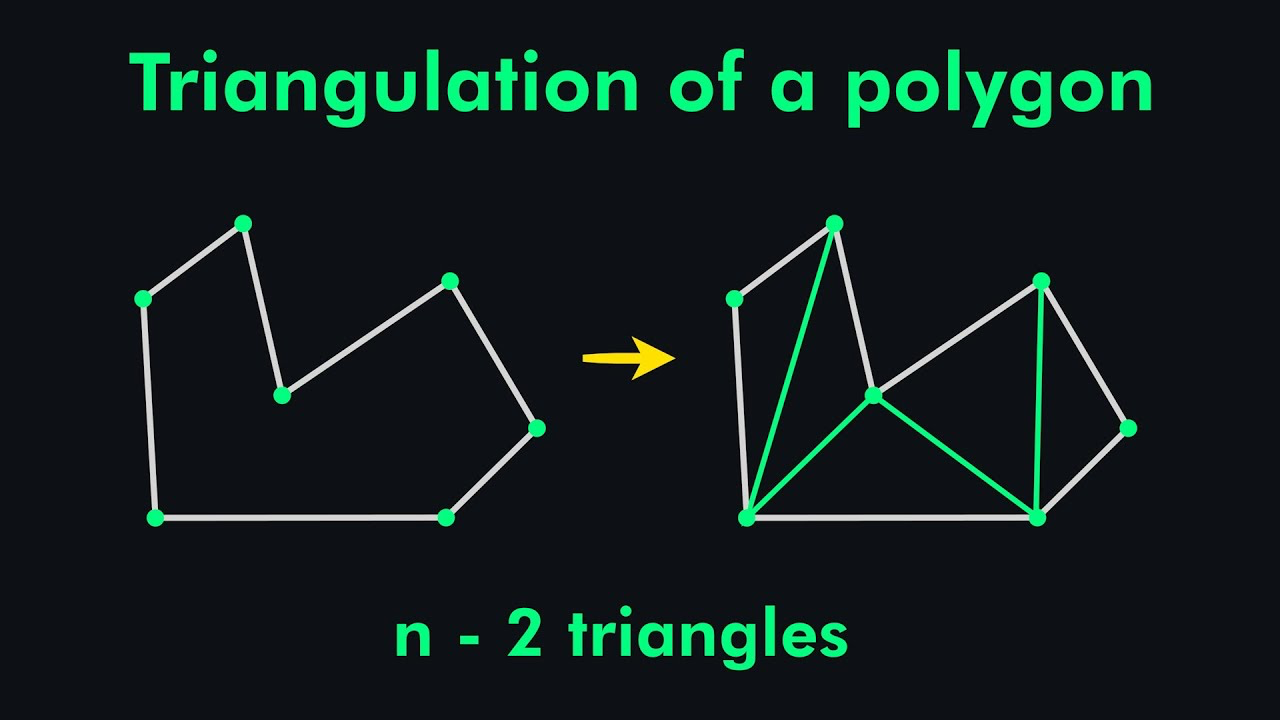
\includegraphics[width=.3\textwidth,align=t]{triangulate}\\\href{https://www.youtube.com/watch?v=2x4ioToqe_c}{Youtube}}
  \end{tabularx}
  
  \begin{solution}
    
  \end{solution}

  \section*{Greedy Algorithms}
\question \href{https://www.vis.uni-stuttgart.de/en/institute/team/Ertl/}{Prof. Dr. rer. nat. Dr. techn. h. c. Dr.-Ing. E. h.} Habib claims that solving the fractional knapsack problem using dynamic programming is overkill. Do you agree with this statement? Justify your claim, i.e. with a supporting argument or a counterexample.

  \begin{solution}
    
  \end{solution}

\question
  \begin{tabularx}{\textwidth}{cX}
    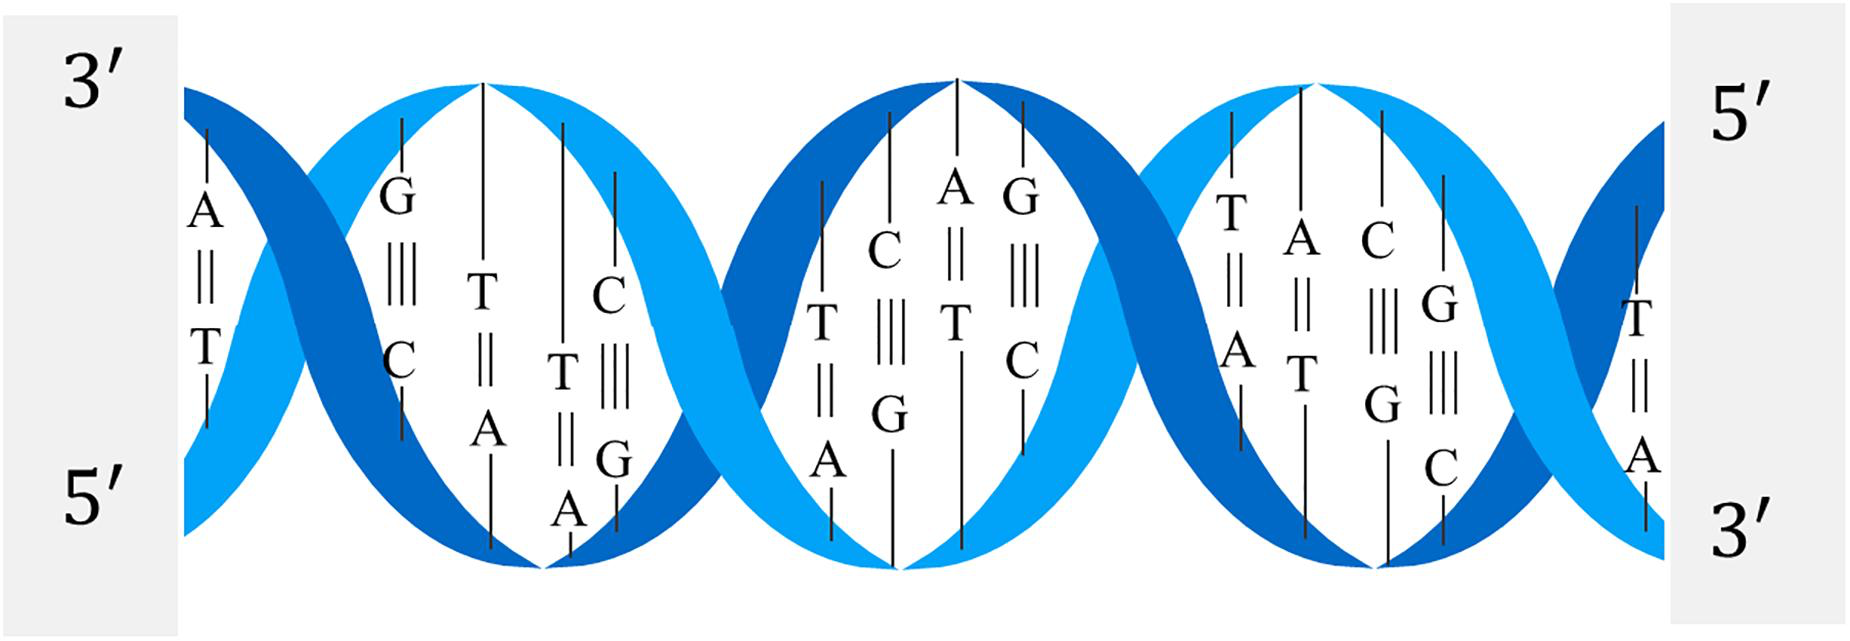
\includegraphics[height=75pt,align=t]{dna}
    &
    Suggest a greedy approach to construct an optimal \href{https://en.wikipedia.org/wiki/Prefix_code}{prefix code}, and argue about its run time complexity? Give the code that your approach computes for the DNA strand, \textit{AATTTAGAAATTCTATTATA}.\\
    \href{https://www.frontiersin.org/articles/10.3389/fbioe.2020.01032/full}{Frontiers}
  \end{tabularx}
  
  \begin{solution}
    
  \end{solution}

\end{questions}

\end{document}

%%% Local Variables:
%%% mode: latex
%%% TeX-master: t
%%% End:
